%  article.tex (Version 3.3, released 19 January 2008)
%  Article to demonstrate format for SPIE Proceedings
%  Special instructions are included in this file after the
%  symbol %>>>>
%  Numerous commands are commented out, but included to show how
%  to effect various options, e.g., to print page numbers, etc.
%  This LaTeX source file is composed for LaTeX2e.

%  The following commands have been added in the SPIE class 
%  file (spie.cls) and will not be understood in other classes:
%  \supit{}, \authorinfo{}, \skiplinehalf, \keywords{}
%  The bibliography style file is called spiebib.bst, 
%  which replaces the standard style unstr.bst.  

\documentclass[]{spie}  %>>> use for US letter paper
%%\documentclass[a4paper]{spie}  %>>> use this instead for A4 paper
%%\documentclass[nocompress]{spie}  %>>> to avoid compression of citations
%% \addtolength{\voffset}{9mm}   %>>> moves text field down
%% \renewcommand{\baselinestretch}{1.65}   %>>> 1.65 for double spacing, 1.25 for 1.5 spacing 
%  The following command loads a graphics package to include images 
%  in the document. It may be necessary to specify a DVI driver option,
%  e.g., [dvips], but that may be inappropriate for some LaTeX 
%  installations. 
\usepackage[]{graphicx}
\usepackage{bm}
\usepackage{amsmath}
\usepackage{nameref}

\newcommand\Tstrut{\rule{0pt}{2.6ex}}         % = `top' strut
\newcommand\Bstrut{\rule[-0.9ex]{0pt}{0pt}}   % = `bottom' strut

\title{Nonlinear Finite Element Analysis Code} 

%>>>> The author is responsible for formatting the 
%  author list and their institutions.  Use  \skiplinehalf 
%  to separate author list from addresses and between each address.
%  The correspondence between each author and his/her address
%  can be indicated with a superscript in italics, 
%  which is easily obtained with \supit{}.

\author{Tyler Ryan \\
	Tyler.Ryan@engineering.ucla.edu
\skiplinehalf
MAE 261B, UCLA \\
March 20, 2015
}

%%%%%%%%%%%%%%%%%%%%%%%%%%%%%%%%%%%%%%%%%%%%%%%%%%%%%%%%%%%%% 
%>>>> uncomment following for page numbers
\pagestyle{plain}    
%>>>> uncomment following to start page numbering at 301 
%\setcounter{page}{301} 
 
\begin{document} 
\maketitle 

\tableofcontents

%%%%%%%%%%%%%%%%%%%%%%%%%%%%%%%%%%%%%%%%%%%%%%%%%%%%%%%%%%%%%
\section{INTRODUCTION}
\label{section: introduction}
This report describes the theory, architecture, implementation, and results of creating a finite element analysis program in the object-oriented programming language of Python (version 3.3.5). A lot of emphasis has been placed on code architecture and verification testing to ensure that the code is easily extensible and robust for future development. In order to get started, we must first understand the equations for and derivations of the fundamental quantities that will lay the foundation for the program. Then we will explore the implementation of these equations into the code architecture and describe some of the key design choices for code structure. Finally, we will discuss the results of implementation by looking at the application of the code to several nonlinear analysis problems. 

\subsection{Curvilinear Coordinates and Frames}
To describe the deformation of an arbitrarily curved body, it is useful to introduce a curvilinear coordinate system that allows us to define a basis in such a way that is natural or convenient for the body. For example, it is easy to describe the deformation of a cylindrical body in cylindrical coordinates, or a spherical body in spherical coordinates. These are idealized examples, but illustrate the point that coordinate axes can be chosen to work well with the geometry of the body undergoing deformation. 

In curvilinear coordinates, we refer to the curved coordinate axes as $\theta^i$, where $i$ ranges from 1 to 3 to represent the three axes. These coordinates are used to describe positions in the body, which will ultimately be expressed in the lab frame. The \textbf{lab frame} can be thought of as the frame of an observer outside of the body, in which positions are described in terms of Cartesian coordinates $x$, $y$, and $z$, or $E_i$. For a given body, we will use curvilinear axes $\theta^i$ in such a way that we can write expressions for $\theta^i$ in terms of $E_i$, and vice versa. 

The curvilinear coordinates are often chose to match the geometry of the body in an \textbf{idealized configuration}. For example, if our body has a shape close to that of a sphere, we would use a sphere as the idealized configuration and spherical coordinates as our curvilinear coordinates. We then define two mappings from the idealized configuration: one to the reference configuration and another to the deformed/current configuration. The \textbf{reference configuration} represents the initial geometry of the body, prior to deformation, and will be represented by capital letter symbols. The \textbf{deformed configuration} represents the geometry of the body at some point in time during deformation, and will be represented with lowercase symbols. This geometry will in general change with time, and thus is often referred to as the current configuration. We can define functions to represent these two mappings in terms of the curvilinear coordinates of the system:

\underline{\textbf{Reference Configuration ($\Omega_0$):}}
\begin{equation}
\bm{X} = \bm{\phi_0}(\theta^i) = f_1(\theta^i)\bm{{e_{\theta_1}}} + f_2(\theta^i)\bm{{e_{\theta_2}}} + f_3(\theta^i)\bm{{e_{\theta_3}}}
\end{equation}

\underline{\textbf{Deformed Configuration ($\Omega$):}}
\begin{equation}
\bm{x} = \bm{\phi}(\theta^i) = g_1(\theta^i)\bm{{e_{\theta_1}}} + g_2(\theta^i)\bm{{e_{\theta_2}}} + g_3(\theta^i)\bm{{e_{\theta_3}}}
\end{equation}

\subsection{Covariant and Contravariant Basis Vectors}
In order to express our reference and deformed configurations, we need to construct bases. Because we are using curvilinear coordinates, we can do this in two ways. The first is to construct the tangent basis vectors, which are tangent to the coordinates axes $\theta^i$. These are referred to as \textbf{covariant basis vectors}, and are denoted with a subscript index as $g_i$. The second is to construct the dual basis vectors, which are normal to the $\theta^i$-surfaces. These surfaces are formed by the plane containing two coordinate axes. For example, the $\theta^1$ surface is the plane containing the $\theta^2$ and $\theta^3$ axes, and the first dual vector will be normal to this surface. These vectors are referred to as \textbf{contravariant basis vectors}, and are denoted with a superscript index as $g^i$. Note that covariant and contravariant basis vector do not in general point in the same direction. 

The covariant and contravariant basis vectors are defined as follows (keeping in mind that capital symbols are used for the reference configuration and lowercase symbols are used for the deformed configuration):
\begin{equation}
\bm{G_i} = \frac{\partial \bm{\phi_0}}{\partial \theta^i}, \quad \bm{G^i} = G^{ij}\bm{G_j}, \quad \bm{g_i} = \frac{\partial \bm{\phi}}{\partial \theta^i}, \quad \bm{g^i} = g^{ij}\bm{g_j},
\end{equation}
where $G^{ij}$ and $g^{ij}$ represent metric tensors, and are described in more detail below. The covariant and contravariant metric tensors are related by the inverse:
\begin{equation}
G^{ij} = [G_{ij}]^{-1}, \quad g^{ij} = [g_{ij}]^{-1}
\end{equation}

\paragraph{Properties}
Because each basis is defined based on three curved axes defined by the geometry of the body, the basis will not in general be orthonormal. In other words, the dot product of two basis vectors will not yield the Kronecker Delta, but will instead give a tensor called the \textbf{metric tensor}.
\begin{equation}
\bm{g_i} \cdot \bm{g_j} = g_{ij} \neq \delta_{ij}, \quad \bm{g^i} \cdot \bm{g^j} = g^{ij} \neq \delta_{ij}
\end{equation}
The elements of the metric tensor $g_{ij}$ describe the length of the tangent vectors (diagonal elements) and the angles between them (off-diagonal elements). Because the bases arises from the curvilinear coordinate axes, it makes sense that the metric tensor does not generally equal the identity matrix. However, the identity matrix is used to describe the relationship between covariant and contravariant basis vectors:
\begin{equation}
\bm{g^i} \cdot \bm{g_j} = \delta^i_j
\end{equation}


\subsection{Kinematic Quantities}
With the basis vectors defined for both the reference, and deformed configurations, we can now compute the kinematic quantities that describe the deformation of the body. 

The \textbf{deformation gradient} is computed from the outer product of basis vectors in the two configurations, and represents the manner in which the body deforms at a given point in space. The diagonal elements represent stretching and the off-diagonal elements represent twisting of the body. 
\begin{equation}
\label{eq: deformation gradient}
\bm{F} = \bm{g_i} \otimes \bm{G^i}
\end{equation}

There are three tensor that describe the strains in the body at a point in space, the \textbf{right Cauchy-Green deformation tensor}, the \textbf{left Cauchy-Green deformation tensor}, and the \textbf{Green-Lagrange Strain}:

\begin{align}
\textrm{Right Cauchy-Green Deformation Tensor:} & \ & \bm{C} 	&= \bm{F}^T\bm{F} & \\
\textrm{Left Cauchy-Green Deformation Tensor:}	& \ & \bm{B}	&= \bm{F}\bm{F}^T & \\
\textrm{Green-Lagrange Strain:}					& \ & \bm{E} 	&= \frac{1}{2}(\bm{C} - \bm{I}) &
\end{align}

\subsection{Constitutive Laws}
\label{subsec: constitutive laws}
The stress-strain relationship for a body is defined by model called a \textbf{constitutive law}. There a various constitutive laws that make different assumptions about the response of a body, such as a material being compressible or incompressible, or behaving elastically or inelastically. In this analysis, we will use the \textbf{Neo-Hookean model}, which assumes hyperelastic material behavior and allows for compression. The law is expressed as an equation for the strain energy density of the body as a function of strain, from which we can derive expression for the \textbf{first Piola-Kirchhoff Stress} and \textbf{tangent moduli}. 

The Neo-Hookean model expresses strain energy density as:
\begin{equation}
\label{eq: strain energy density}
w(\bm{C}) = \frac{\lambda_0}{2}[ln(J)]^2 - \mu_0 ln(J) + \frac{\mu_0}{2}(tr(\bm{C}) - 3),
\end{equation}
where $J = det(\bm{F})$ is referred to as the \textbf{Jacobian}, and $\lambda_0$ and $\mu_0$ are the \textbf{first lam\'e parameter} and \textbf{shear modulus} of the material, respectively. The strain energy density can be rewritten entirely as a function of the deformation gradient $\bm{F}$ by expressing $tr(\bm{C})$ in terms of $\bm{F}$:
\begin{gather*}
tr(\bm{C}) = C_{kk} = C_{kl}\delta_{kl} \\
C_{kl} = (F_{km})^T(F_{ml}) = F_{mk}F_{ml} \\
\implies tr(\bm{C}) = F_{mk}F_{ml}\delta_{kl}
\end{gather*}
Now we can derive an expression for the first Piola-Kirchhoff stress $P_{ij}$:
\begin{align}
P_{ij} 	&= \frac{\partial w}{\partial F_{ij}} = \frac{\partial}{\partial F_{ij}} \left[\frac{\lambda_0}{2}ln^2(J) - \mu_0 ln(J) + \frac{\mu_0}{2}(F_{mk}F_{ml}\delta_{kl} - 3)\right] \\
		&= \lambda_0 ln(J) \left(\frac{1}{J}\right) \frac{\partial J}{\partial F_{ij}} - \mu_0 \left(\frac{1}{J}\right) \frac{\partial J}{\partial F_{ij}} + \frac{\mu_0}{2} \left[\frac{\partial F_{mk}}{\partial F_{ij}} F_{ml} \delta_{kl} + F_{mk} \frac{\partial F_{ml}}{\partial F_{ij}} \delta_{kl}\right]
\end{align}
Using the identity $\frac{\partial J}{\partial F_{ij}} = J F^{-1}_{ji}$:
\begin{align}
P_{ij} 	&= \lambda_0 ln(J) \left(\frac{1}{J}\right) (J F^{-1}_{ji}) - \mu_0 \left(\frac{1}{J}\right) (J F^{-1}_{ji}) + \frac{\mu_0}{2} \left[\delta_{mi}\delta_{kj} F_{ml} \delta_{kl} + F_{mk} \delta_{mi}\delta_{lj} \delta_{kl}\right] \\
		&= \lambda_0 ln(J) F^{-1}_{ji} - \mu_0 F^{-1}_{ji} + \frac{\mu_0}{2} \left[\delta_{mi}\delta_{kj} F_{mk} + F_{ml} \delta_{mi}\delta_{lj}\right] \\
		&= \lambda_0 ln(J) F^{-1}_{ji} - \mu_0 F^{-1}_{ji} + \frac{\mu_0}{2} \left[F_{ij} + F_{ij}\right] \\
		&= \left[\lambda_0 ln(J) - \mu_0 \right]F^{-1}_{ji} + \mu_0 F_{ij}
\end{align}
We can take another derivative with respect to the deformation gradient to find the tangent moduli $C_{ijkl}$:
\begin{align}
C_{ijkl} 	&= \frac{\partial P_{ij}}{\partial F_{kl}} \\
			&= \frac{\partial}{\partial F_{kl}} \left[\left[\lambda_0 ln(J) - \mu_0 \right]F^{-1}_{ji} + \mu_0 F_{ij}\right] \\
			&= \lambda_0 \left(\frac{1}{J}\right) \frac{\partial J}{\partial F_{kl}} F^{-1}_{ji} + \left[\lambda_0 ln(J) - \mu_0 \right] \frac{\partial F^{-1}_{ji}}{\partial F_{kl}} + \mu_0 \frac{\partial F_{ij}}{\partial F_{kl}}
\end{align}
Using the identity $\frac{\partial F^{-1}_{ji}}{\partial F_{kl}} = -F^{-1}_{jk} F^{-1}_{li}$:
\begin{align}
C_{ijkl}	&= \lambda_0 \left(\frac{1}{J}\right) (J F^{-1}_{lk}) F^{-1}_{ji} + \left[\lambda_0 ln(J) - \mu_0 \right]\left(-F^{-1}_{jk} F^{-1}_{li}\right) + \mu_0 \delta_{ik}\delta_{jl} \\
			&= \lambda_0  F^{-1}_{lk} F^{-1}_{ji} - \left[\lambda_0 ln(J) - \mu_0 \right] F^{-1}_{jk} F^{-1}_{li} + \mu_0 \delta_{ik}\delta_{jl}
\end{align}

To summarize, we now have the following three expressions for the Neo-Hookean constitutive law in terms of the deformation gradient $\bm{F}$:
\begin{align}
\textrm{Strain Energy Density:}			& \ & w(\bm{F}) &= \frac{\lambda_0}{2}[ln(J)]^2 - \mu_0 ln(J) +
															\frac{\mu_0}{2}(tr(\bm{F}^T\bm{F}) - 3) & \\
\textrm{First Piola-Kirchhoff Stress:} 	& \ & P_{ij} 	&= \left[\lambda_0 ln(J) - \mu_0 \right]F^{-1}_{ji} + \mu_0 F_{ij}
															& \\
\textrm{Tangent Moduli:}				& \ & C_{ijkl}	&= \lambda_0  F^{-1}_{lk} F^{-1}_{ji} - \left[\lambda_0 ln(J) -
															\mu_0 \right] F^{-1}_{jk} F^{-1}_{li} + \mu_0 \delta_{ik}\delta_{jl} &
\end{align}

\subsection{Plane Stress}
The assumption of plane stress places a constraint on the structure of the deformation gradient as well as the first Piola-Kirchhoff stress tensor. For this example, say we have a thin plate with the thickness aligned with the third coordinate axis. Then the deformation gradient should have no out of plane shear components, and a stretch component $\lambda$ in the 3-direction to account for the fact that there may be some strain through the thickness:
\begin{equation}
\bm{F} = 
\begin{bmatrix}
F_{11} 	& F_{12} 	& 0 \\
F_{21} 	& F_{22} 	& 0 \\
0   	& 0			& \lambda	
\end{bmatrix}
\end{equation}
The first Piola-Kirchhoff stress tensor should have a value of 0 for $P_{33}$. Since the only arbitrary or prescribed quantities of $\bm{F}$ are the $2 \times 2$ matrix of in-plane elements, we say that $P_{33}$ is a function only of $F_{\alpha\beta}$ (where $\alpha$ and $\beta$ each run from 1 to 2) and $\lambda$ (referred to as the \textbf{stretch ratio}):
\begin{equation}
P_{33}(F_{\alpha\beta}, \lambda) = 0
\end{equation}  
Because $F_{\alpha\beta}$ is prescribed, we must solve this equation by finding the value of $\lambda$ that makes it true. $\bm{P}(\bm{F})$ is nonlinear, and therefore must be solved iteratively using Newton's Method. 

\subsubsection{Newton's Method}
\textbf{Newton's Method} is an iterative technique for solver a nonlinear equation $f(\lambda)$. To use it, we must start by choosing a reasonable initial value for $\lambda$ for which $f(\lambda)$ likely does not equal zero. 
\begin{equation}
f(\lambda_0) \neq 0
\end{equation}
Then we will perturb $\lambda$ by some small quantity, and use a first order Taylor approximation to solve for the value of the perturbation that will make $f(\lambda)$ equal to zero.
\begin{equation}
\label{eq: dlambda}
f(\lambda + d\lambda) = f(\lambda) + \frac{df(\lambda)}{d\lambda}d\lambda = 0 \implies d\lambda = -\left(\frac{df(\lambda)}{d\lambda}\right)^{-1} f(\lambda)
\end{equation}
We then use this perturbation to compute a new value of $\lambda$ and repeat the process. This loop will continue until $f(\lambda)$ is within some tolerance of 0, at which point we say the loop \textbf{converges}. It is very important to note that if $\lambda_0$ is far enough from the final value of $\lambda$, this loop will \textbf{diverge}. In later reports, we will explore in more detail the techniques used to ensure good initial guesses. 

For the plane stress application, the function we are attempting to solve iteratively is $P_{33}(F_{\alpha\beta}, \lambda) = 0$. Therefore we can express equation \ref{eq: dlambda} in terms of the quantities of our problem as:
\begin{equation}
\label{eq: dlambda P}
d\lambda = - (C_{3333})^{-1} P_{33}(F_{\alpha\beta}, \lambda)
\end{equation}

\subsubsection{2D Tangent Moduli}
The plane stress assumptions serves to simplify the problem by reducing dimension from 3D to 2D. Once we have solved for lambda using Newton's method, we can now proceed with the analysis using reduced matrices containing only the in-plane components. First, note that 2D and 3D strain energy density are defined to be equal. For the first Piola-Kirchhoff stress, the transition to 2D is simple, because all components in the 3-direction have been forced to zero under the assumption of plane stress. Therefore, the in-plane components of $\bm{P}$ are nothing more than the $2 \times 2$ matrix containing the non-zero elements. In other words, $P_{\alpha\beta}$ is subset of $P_{ij}$. For the tangent moduli however, the transition is not that simple. Despite imposing plane stress, there will in general be non-zero elements in the 3-directions, and we cannot simply reduce to 2D by taking a subset of this tensor. Instead, we want to capture the contributions of these non-zero elements by created an adjusted 2D 4th order tensor from the full 3D tangent moduli. The components of the 2D tangent moduli can be found in the following way:
\begin{equation}
P^{2D}_{\alpha\beta} \equiv \frac{\partial w^{2D}}{\partial F_{\alpha\beta}} = \frac{\partial}{\partial F_{\alpha\beta}}
						\left[ w(F, \lambda) \right] = \frac{\partial w}{\partial F_{\alpha\beta}} + \frac{\partial w}{\partial \lambda} \frac{\partial \lambda}{\partial F_{\alpha\beta}}
\end{equation}
We know that $\frac{\partial w}{\partial F_{\alpha\beta}} = P_{\alpha\beta}$ and $\frac{\partial w}{\partial \lambda} = 0$, so we can write:
\begin{equation}
P_{\alpha\beta} = \frac{\partial w(F_{\alpha\beta}, \lambda)}{\partial F_{\alpha\beta}}, \quad P^{2D}_{\alpha\beta} = P_{\alpha\beta}
\end{equation}
This shows, as stated previously, that the 2D form of the first Piola-Kirchhoff stress is just a subset of the 3D form. Now we can use this to compute the tangent moduli:
\begin{equation}
C^{2D}_{\alpha\beta\delta\gamma}	\equiv \frac{\partial P^{2D}_{\alpha\beta}}{\partial F_{\delta\gamma}} =
										\frac{\partial^2 w^{2D}}{\partial F_{\alpha\beta}F_{\delta\gamma}} =
										\frac{\partial}{\partial F_{\delta\gamma}} \left[P_{\alpha\beta}(F_{\alpha\beta}, \lambda)\right] =
										\frac{\partial P_{\alpha\beta}}{\partial F_{\delta\gamma}} + \frac{\partial P_{\alpha\beta}}{\partial \lambda} \frac{\partial \lambda}{\partial F_{\delta\gamma}}
\end{equation}
We know that $\frac{\partial P_{\alpha\beta}}{\partial F_{\delta\gamma}} = C_{\alpha\beta\delta\gamma}$ and $\frac{\partial P_{\alpha\beta}}{\partial \lambda} = \frac{\partial P_{\alpha\beta}}{\partial F_{33}} = C_{\alpha\beta 3 3}$, so we can write:
\begin{equation}
C^{2D}_{\alpha\beta\delta\gamma} = C_{\alpha\beta\delta\gamma} + C_{\alpha\beta 3 3} \frac{\partial \lambda}{\partial F_{\delta\gamma}}
\end{equation}
Now we can find $\frac{\partial \lambda}{\partial F_{\delta\gamma}}$ by enforcing the plane stress assumption that $P_{33}(F_{\alpha\beta}, \lambda) = 0$. 
\begin{equation}
P_{33}(F_{\alpha\beta}, \lambda) = 0 \implies dP_{33} = 0 = \frac{\partial P_{33}}{\partial F_{\alpha\beta}} dF_{\alpha\beta} + \frac{\partial P_{33}}{\partial F_{33}} d\lambda
\end{equation}
\begin{align}
0 &= C_{3 3 \alpha\beta} dF_{\alpha\beta} + C_{3333} d\lambda \\
0 &= C_{3 3 \alpha\beta} dF_{\alpha\beta} + C_{3333} \frac{\partial \lambda}{\partial F_{\alpha\beta}} dF_{\alpha\beta} \\
0 &= \left( C_{3 3 \alpha\beta} + C_{3333} \frac{\partial \lambda}{\partial F_{\alpha\beta}} \right) dF_{\alpha\beta}
\end{align}
\begin{equation}
\implies \frac{\partial \lambda}{\partial F_{\alpha\beta}} = - \frac{C_{3 3 \alpha\beta}}{C_{3333}}
\end{equation}
Now we can use this value to solve for the components of the 2D tangent moduli:
\begin{align}
C^{2D}_{\alpha\beta\delta\gamma} &= \frac{\partial}{\partial F_{\delta\gamma}} \left[ P_{\alpha\beta}(F_{\alpha\beta},
									\lambda)\right] = C_{\alpha\beta\delta\gamma} + C_{\alpha\beta 3 3} \frac{\partial \lambda}{\partial F_{\delta\gamma}} \\
& \implies C^{2D}_{\alpha\beta\delta\gamma} = C_{\alpha\beta\delta\gamma} - C_{\alpha\beta 3 3} C_{3 3 \delta\gamma} \left(\frac{1}{C_{3333}}\right)
\label{eq: 2d tangent moduli}
\end{align}
Using this equation we can compute the adjusted 2D tangent moduli under the assumption of plane stress from the components of the full 3D tangent moduli. 

\subsection{Finite Elements}
\label{sec: finite elements}
In order to analyze the behavior of body, we must discretize the domain into finite elements. These elements can in general have any number of sides, but triangles and quadrilaterals provide more than enough flexibility and are much simpler to work with. In this analysis, we will focus on the use of triangular elements. When a domain in broken up into triangular elements, each triangle will in general have different dimensions and different orientations. For this reason it becomes very useful to map each general element into an isoparametric element.

\textbf{Isoparametric elements} are standard elements defined in a natural coordinate system for which we can use shape functions to interpolate the behavior of the element between nodes. An example of an isoparametric triangular element is shown in figure \ref{fig: isoparametric triangular element}. The element is bounded by nodes, and the shape functions define the shape of the body between them. Shape functions relate the coordinates of every point in the element to the positions of the nodes, allowing for interpolation of values such as displacement within the element.

\begin{figure}[h]
	\centering
	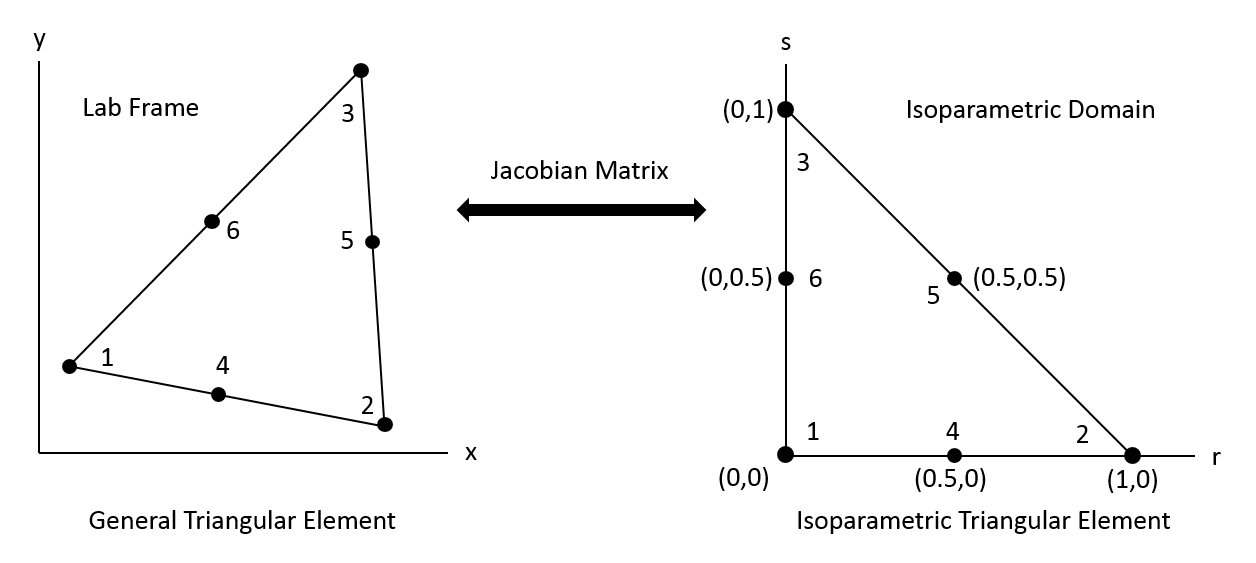
\includegraphics[width=7in]{isoparametric_triangular_element.png}
	\caption{A general triangular element is mapped to an isoparametric triangular element by the Jacobian matrix. A linear triangular element uses only nodes 1-3, removing the midpoint nodes. A quadratic triangular element uses all 6 nodes.} 
	\label{fig: isoparametric triangular element}
\end{figure}

The finite element analysis is driven by nodal positions, as the behavior of each element is dependent entirely on the behavior of the nodes. Depending on the desired accuracy, 3-node or 6-node triangular elements may be used. A 3-node triangular element is considered linear, as there is no information between the nodes to allow for curving. Thus the 6-node triangular element is considered quadratic, as the midpoint nodes along the edge allow for nonlinear behavior. For each of these element types, there are a number of shape functions equal to the number of nodes, and every isoparametric element is characterized by these same functions.

A location in the natural coordinate system $(r,x)$ can be interpolated from the lab frame nodal positions $(x,y)$ by the shape functions:
\begin{equation}
\label{eq: shape function mapping}
\bm{x}(r,s) = \sum\limits_{a} N_a(r,s) \bm{x}_a
\end{equation}
where $a$ is indexing the nodes. 

\subsubsection{Jacobian Matrix}
The general element is mapped from the lab frame to the isoparametric domain by the \textbf{Jacobian matrix}. The Jacobian matrix is based on the reference nodal positions and the shape functions, and can be expressed as:
\begin{equation}
\label{eq: Jacobian matrix}
J_{I\alpha} = \sum\limits_{a} X_{ia} N_{a,\alpha}
\end{equation}
where $X_{ia}$ are the components of the reference nodal position vectors. The Jacobian matrix has dimensions of (lab frame dimensions) $\times$ (element dimensions). In this analysis, the plane stress assumption will allow for the use of two dimensional elements deforming in a three dimensional lab frame. Therefore the Jacobian matrix will be 3 $\times$ 2. 

With the Jacobian matrix, we have a means for moving between the isoparametric and physical domains, and it will be used in the calculations for numerous quantities that describe the behavior of the element.

\subsubsection{Element Behavior}
With the Jacobian matrix defined, the deformation gradient can now be computed in alternative manner to using the basis vectors of the reference and current configurations as defined in equation \ref{eq: deformation gradient}. Using the nodal positions in the current configuration $x_{ia}$, and the information about the current configuration carried by the Jacobian matrix, the \textbf{deformation gradient} can be expressed as:
\begin{equation}
\label{eq: deformation gradient using Jacobian matrix}
F_{ij} = \sum\limits_{a} x_{ia} N_{a,\alpha} J_{\alpha j}^{-1}
\end{equation}
With the deformation gradient and material response quantities from the constitutive model, three quantities can be computed: strain energy, internal nodal force array, and the stiffness matrix. These quantities describe the behavior of the entire element by integrating the material response quantities over the element domain. Here the isoparametric formulation comes in handy because the integral can be performed in the isoparametric domain and then transformed back to the physical domain using the inverse Jacobian matrix. These integrals are computed using a numerical integration technique called Gauss quadrature, which will be discussed in detail in section \textit{\nameref{sec: gauss quadrature}}. 

The \textbf{strain energy} of the element is determined by integrating the strain energy density:
\begin{equation}
\label{eq: strain energy}
W = \int\limits_{\Omega_0} w dV
\end{equation}

The \textbf{internal nodal force array} is the representation of a distributed force over the element at the nodes. In other words, the distributed load is converted to a set of equivalent forces acting only on the nodes of the element. The force array is determined by integrating the first Piola-Kirchhoff stress:
\begin{equation}
\label{eq: internal nodal force array}
f_{ia}^{int} = \int\limits_{\Omega_0} P_{ij} N_{a,\alpha} J_{\alpha j}^{-1} dV
\end{equation}

The \textbf{stiffness matrix} represents the resistance of the element to deformation in various directions. It is determined by integrating the two dimensional tangent moduli that has been adjusted for plane stress:
\begin{equation}
\label{eq: stiffness matrix}
K_{iakb} = \int\limits_{\Omega_0} C_{ijkl}^{2D} N_{a,\alpha} N_{b,\beta} J_{\alpha j}^{-1} J_{\beta l}^{-1} dV
\end{equation}

\subsubsection{Gauss Quadrature}
This analysis requires the evaluation of integrals, and it would be costly to perform integration explicitly. For this reason, we will use Gauss quadrature to perform numerical integration. Gauss quadrature works by using a weighted sum of function values at specific quadrature points within a domain. It is constructed to yield exact results for polynomial functions of degree $2n-1$ or lower for n-point quadrature, provided that the polynomial is well-approximated at the quadrature points. In this analysis, we will make use of 1-point quadrature, which will evaluate a linear polynomial exactly, and 3-point quadrature, which will evaluate a fifth order polynomial exactly. 

Whether or not the function is well-approximated at the quadrature points will be determined by whether the interpolated shape function values at these points can capture the element behavior. For example, for a 3-node isoparametric triangular element, 1-point quadrature will provide exact integration results, as the element can only display linear behavior, which will be exactly interpolated by the shape functions. In order to accurately capture quadratic behavior, a 6-node element must be used to pick up the behavior between corner nodes. We must also use 3-point quadrature to ensure accuracy, because the accuracy 1-point quadrature is limited to linear functions.

The computational cost will be lowest for the lowest order to quadrature, therefore the analysis will make use of the lowest order quadrature possible to ensure accurate results. There are applications for intentionally using lower-order quadrature, but these will not be discussed here.

The general expression for Gauss quadrature of a function $g(\zeta)$ is:
\begin{equation}
\label{eq: Gauss quadrature general}
\int\limits_{-1}^{1} g(\zeta)d\zeta = \sum\limits_{i=1}^{n} g(\tilde{\zeta}_i) w_i
\end{equation}
where $n$ is the number of quadrature points, $\tilde{\zeta}_i$ is the coordinate of the $i$th quadrature point, and $w_i$ is the weight of the $i$th quadrature point. 

The application of this equation in the analysis is further discussed in \textit{\nameref{sec: quadrature}}.


%%%%%%%%%%%%%%%%%%%%%%%%%%%%%%%%%%%%%%%%%%%%%%%%%%%%%%%%%%%%%
\section{CODE ARCHITECTURE \& FORMULATION OF NUMERICAL METHODS} 

I have put in a lot of effort to ensure that the initial code base is structured to be robust and extensible to future developments. This means that future work will involve adding more to the existing classes and functions rather than rewriting them. I have done my best to take full advantage of Python as an object-oriented project language to create an architecture that makes sense according to the current state of my evolving understanding of finite element analysis. I will describe my code at the highest level before discussing the details of implementation.

\subsection{Code Architecture}
My goal is to structure the model such that its inputs are provided in an intuitive format that is repeatable for any application. Whether running a simple verification test or a full deformation analysis on a body, the inputs should only differ in their values and the desired output information requested.

\subsubsection{Brief Module Descriptions}
\begin{description}
	\item[constants.py] integers and strings used throughout the model such they can be conveniently referenced without having to hard-code their values into the model.
	\item[constitutive\_models.py] contains classes for each constitutive law (ie. Neo-Hookean), each of which contains methods for computing the values of strain energy density, first Piola-Kirchhoff stress, and tangent moduli.
	\item[deformation\_gradient.py] deformation gradient class which defines and updates the deformation of the body under specified assumptions.
	\item[elements.py] contains the different types of isoparametric elements available for use in analysis, including the 3 and 6-node triangular elements. Also contains methods for updating element-level properties such as strain energy. 
	\item[exceptions.py] errors that are raised during the analysis (usually from the tests module) in the event of an incorrect or unexpected result, or some kind of violation that indicates a breaking of physical laws or constraints.
	\item[frames.py] contains classes for the frames/configurations and the basis vectors.
	\item[kinematics.py] functions that compute the strain tensors from the deformation gradient. 
	\item[materials.py] contains classes for different material options, each of which contains the properties of the material.
	\item[model.py] contains the finite element model, the master class that manages the analysis and keeps track of the highest level information. 
	\item[model\_io\_\#.py] this is the module from which the model is set up and run, and is the only file a user will interact with. 
	\item[operations.py] commonly used functions, such as Newton's Method, or the generation of a random deformation gradient for testing purposes. 
	\item[nodes.py] contains node classes that keep track of reference and current positions, as well as local and global IDs for assembly purposes. 
	\item[quadrature.py] contains parameters for one and three point Gauss quadrature, as well as a quadrature point class that contains properties for material response values. 
	\item[tests.py] verification test functions that ensure the accuracy of the code and check for physical violations.
\end{description}

\subsubsection{Finite Element Model}
The highest level object in the analysis is the Model class, or the Finite Element Model. This is the "master" of the analysis, and is responsible for keeping track of globally needed information as well as setting up and running the analysis. The model keeps track of the material, constitutive model, quadrature class, and element type. It is also responsible for creating the nodes and elements, and performing the global assembly. It stores lists of all element and node objects in the analysis to allow for easy iteration downward from the model level when updating the current configuration. 

\paragraph{Model Setup}
Elements are the building blocks of the model, and are composed of nodes and quadrature points. Nodes define the mesh that discretizes the domain of the body, and belong to multiple parent elements. For this reason, nodes are created first by the model through a meshing function (TO BE ELABORATED ON LATER) and assigned a reference position, a list of parent elements, and both local and global IDs. The reference position defines the position of the node in the reference configuration. The list of parent elements defines the element objects the node belongs to. The local ID keeps track of the node number 1-6 within an element as shown in figure \ref{fig: isoparametric triangular element}. Therefore many nodes will share local IDs, creating the need for a global ID, which creates a unique identifier for the node within the model.

Once the nodes are created, they are assigned to their parent elements, who store a list of their nodes. With nodes assigned, the elements then create their quadrature point(s) based on the quadrature class selected by the model and then perform the one-time calculation of the Jacobian matrix from the reference nodal positions. The primary advantage of using isoparametric elements is that once the general elements have been mapped to the isoparametric domain by the Jacobian matrix, every element can be treated identically.

This process can be summarized by the order of method calls, shown here:
\begin{enumerate}
	\item model.create\_mesh (TO BE ADDED LATER)
	\subitem model.create\_nodes
	\subitem model.create\_elements
	\item model.assign\_nodes
	\item element.create\_quadrature\_points (for each element)
	\subitem element.calculate\_jacobian\_matrix
\end{enumerate}

\paragraph{Updating the Current Configuration}
For each step of deformation, the model must update its current configuration. To do this, the model iterates through each element, which in turn iterates through its nodes, and updates their current position. With the current nodal positions defined, each element can use its shape functions to update the deformation gradient at each of its quadrature points. Each quadrature point then uses its deformation gradient to compute the material response from the constitutive law. With the quadrature point quantities fully defined, each element can use gauss quadrature to integrate over the element and compute values for the strain energy, force array, and stiffness matrix. 

This process can be summarized by the order of method calls, shown here:
\begin{enumerate}
	\item model.update\_current\_configuration
	\item element.update\_current\_configuration (for each element)
	\item node.update\_current\_position (for each node in the element)
	\item quadrature\_point.update\_deformation\_gradient (for each quadrature point in the element)
	\item deformation\_gradient.update\_F (for the deformation gradient of each quadrature point in the element)
	\item deformation\_gradient.enforce\_plane\_stress (for the deformation gradient of each quadrature point in the element)
	\item quadrature\_point.update\_material\_response (for each quadrature point in the element)
	\item element.update\_strain\_energy (for each element)
	\item element.update\_force\_array (for each element)
	\item element.update\_stiffness\_matrix (for each element)
\end{enumerate}


\subsection{Implementation and Verification Tests}
In this section, I will describe the key design choices made with regards to implementation, and in particular how these relate to the verification tests that ensure the correctness of the code and validity of the analysis. 

\subsubsection{Assembly}
% TODO
To be elaborated on in final report. 

\subsubsection{Numerical Differentiation}
The model uses many equations that require the programming of hand computed derivatives. In order to ensure correctness of derivatives, the results can be compared against the results of numerical differentiation.

The numerical differentiation test uses the 3-point formula to check the validity of our computed results for the first Piola-Kirchhoff and the tangent moduli. The 3-point formula comes from a 3rd order Taylor expansion, and is given by:
\begin{gather}
\label{eq: 3 point formula}
f'(a) \approx \frac{f(a + h) - f(a - h)}{2h} \equiv f'_h(a) \\[1ex]
\textrm{Error} = f'_h(a) - f'(a) < TOLERANCE \implies pass
\end{gather}
The perturbation $h$ is applied element by element, and the approximated value is compared to the exact value computed from the constitutive law to ensure that they are within tolerance of each other. The tolerance is necessary because the two values will not be an exact match, and there is an expected error from the Taylor expansion on the order of $h^2$. 

\subsubsection{Elements}
Elements are implemented as classes that inherit from a base element class that contains all necessary properties for defining an element as well as the necessary methods for analysis. Element properties include dimension, node\_quantity, and node\_positions, all of which are defined based on element type. 

The element class defines the nodal positions in the isoparametric domain, and the order of node objects in the nodes list will match the ordering for the isoparametric element (ie. 1-3 are corner nodes, 4-6 are midpoint nodes, see figure \ref{fig: isoparametric triangular element}). This order is important such that the Jacobian matrix mapping makes physical sense. 

The element class also contains the material quantities that include the strain energy, force array, and stiffness matrix, which are updated for every deformation. 

\paragraph{Tests}
The force array and stiffness matrix are the first and second derivative of the strain energy, respectively. Their values are checked against numerical differentiation using the 3-point formula from equation \ref{eq: 3 point formula}. In this case, it is the current nodal positions that are perturbed, which in turn creates a perturbed deformation gradient at each quadrature point, which leads to perturbed strain energy densities and therefore a perturbed strain energy and force array. For this reason, strain energy and force array will appear as functions of current nodal position to make this point clear:
\begin{align}
(F_h)_{ia} &= \frac{W(x_{ia} + h) - W(x_{ia} - h)}{2h} \\[1ex]
(K_h)_{iakb} &= \frac{F_{ia}(x_{kb} + h) - F_{ia}(x_{kb} - h)}{2h}
\end{align}

\subsubsection{Shape Functions}
The element classes contains predefined shape functions and shape function derivatives as class methods for each element type that return values at a given location in the isoparametric domain. The shape functions are defined inside the element classes because they are specific to element type and number of nodes.

\paragraph{Tests}
The shape function derivatives are verified using the 3-point formula from equation \ref{eq: 3 point formula}. For derivatives with respect to coordinate $r$, the $r$ position of the shape function is perturbed, and likewise for $s$ derivatives:
\begin{align}
\frac{\partial N}{\partial r} &= \frac{N(r + h, s) - N(r - h, s)}{2h} \\[1ex]
\frac{\partial N}{\partial s} &= \frac{N(r, s + h) - N(r, s - h)}{2h}
\end{align}

Shape functions also have the important properties of satisfying partition of unity, partition of nullity, and completeness. Partition of unity that the sum of the shape functions at any point in the isoparametric domain must sum to 1. Therefore, each element type must be tested such that its shape functions satisfy:
\begin{equation}
\label{eq: partition of unity}
\sum\limits_{a} N_a(r,s) = 1
\end{equation}

Additionally, the shape function derivatives must satisfy the partition of nullity, or that they must sum to 0 at any point in the domain:
\begin{equation}
\label{eq: partition of nullity}
\sum\limits_{a} N_{a,\alpha}(r,s) = 0
\end{equation}

Finally the shape functions must be complete, meaning that they can interpolate a random linear polynomial $p$ exactly. This means that the value of a $p$ at a random point in the domain $\bm{\theta^*}$ should be exactly equal to the value interpolated by the shape functions using the values of $p$ at the nodes $p(\bm{\theta_a})$. We can define a random linear polynomial as:
\begin{equation}
p(\bm{\theta}) = \sum\limits_{|\alpha| \leq 1} a_{\alpha}\theta^{\alpha}
\end{equation}
where $a_{\alpha}$ are random coefficients. Now we can check that the value of the polynomial at a random point is equal to the interpolated values as:
\begin{equation}
\label{eq: completeness}
p(\bm{\theta^*}) = \sum\limits_{a} p(\bm{\theta}_a) N_a(\bm{\theta^*})
\end{equation}

\subsubsection{Nodes}
Nodes are implemented as classes. There are two types of nodes that inherit from a base node class: CornerNode and MidpointNode. Both have an identical set of properties, including:
\begin{itemize}
	\item local ID
	\item global ID
	\item reference position
	\item current position
	\item list of parent elements
\end{itemize} 

The reason why these two classes are separated is solely for the purpose of identification. When the mesh is created, the corner nodes define the element boundaries, and the midpoint nodes are not created until the mesh is complete. (ELABORATE IN FINAL REPORT). 

\subsubsection{Quadrature}
\label{sec: quadrature}
There are quadrature classes for one-point and three-point quadrature with properties that define the number of quadrature points, and their positions and weights. The quadrature point class is used to create the quadrature point objects that are assigned to each element for the purposes of numerical integration using Gauss quadrature. Each object has a position and a weight based on the quadrature class being used by the model, and has properties for the quadrature point-level quantities described in \textit{\nameref{sec: property levels}}. 

\paragraph{Gauss Quadrature}
Gauss quadrature is carried out in the element methods that evaluate the strain energy, force array, and stiffness matrix.

Because this analysis will make use of isoparametric triangular element under the plane stress assumption, the bounds of integration must be adjusted from equation \ref{eq: Gauss quadrature general}, and the integral must be made two dimensional. The following will be the expression implemented in the code for numerical integration (written for 2-tensor but would be the same form for a different order) over the isoparametric element domain:
\begin{equation}
\label{eq: Gauss quadrature}
\int\limits_{0}^{1} \int\limits_{0}^{1-s} G_{ij}(r,s)dr ds \approx \frac{1}{2} \sum\limits_{k=1}^{n} G_{ij}(r_k,s_k) w_k
\end{equation}

\subsubsection{Property Levels}
\label{sec: property levels}
It is important to distinguish the level at which certain key quantities in the analysis are defined. There are three levels we are concerned with: model-level, element-level, and quadrature point-level. At each of these levels, some quantities are defined or computed one time, and others are updated with every deformation step. This information is summarized here:

\noindent
\textbf{Model:}
\begin{itemize}
	\item material
	\item constitutive model
	\item quadrature class
	\item element type
\end{itemize}

\noindent
\textbf{Element:} \smallbreak
\indent \textit{One-time:}
\begin{itemize}
	\item Jacobian matrix
\end{itemize}
\smallbreak \textit{Every step:}
\begin{itemize}
	\item strain energy
	\item internal nodal force array
	\item stiffness matrix
\end{itemize}

\noindent
\textbf{Quadrature Point:} \smallbreak
\textit{One-time:}
\begin{itemize}
	\item position
	\item weight
\end{itemize}
\smallbreak \textit{Every step:}
\begin{itemize}
	\item deformation gradient
	\item strain energy density
	\item first Piola-Kirchhoff stress
	\item tangent moduli
\end{itemize}


\subsubsection{Deformation Gradient}
The deformation gradient is extremely important, as it is the driver for all kinematics and material response. Therefore, if we begin our analysis with a deformation that does not make physical sense, then neither will our results. For this reason, I decided to make the deformation gradient be represented by a class rather than by a simple $3 \times 3$ matrix. Each time a deformation gradient is initialized with its matrix values as one of its attributes, it immediately computes and checks the value of the Jacobian. For the deformation gradient to have physical meaning, the Jacobian must be greater than zero, otherwise there is some unphysical inversion of the body taking place. If the Jacobian is negative, an error is raised to indicate this, and the analysis is halted. This ensures that an unphysical deformation gradient never makes it past initialization. 

This quantity is also unique in that its structure is directly affected by the assumption of plane stress. So if the deformation gradient is initialized with this assumption, it will immediately enforce it by computing the value for the unknown stretch ratio using Newton's Method (more detail on this later), and then again checking the value of the Jacobian from the finalized matrix to ensure validity.

Similarly, the class also contains a method for enforcing plane strain, but this has not yet been implemented. 

\subsubsection{Constitutive Laws}
The model keeps a reference to the constitutive law object being using for the analysis. As of now, there is only one option, and that is the Neo-Hookean model. The constitutive law is nothing more than a set of three methods that compute the material response from a $3 \times 3$ deformation gradient. The expressions for these quantities are computed by hand such that derivatives do not need to be handled in the code, as this would be very difficult. The class has no knowledge of the assumptions of the model (ie. plane stress/strain), as this information is contained in the construction of the deformation gradient itself, and therefore the return values will reflect this assumption without being aware of it. 

The methods for first Piola-Kirchhoff stress and tangent moduli contain two optional parameters: the requested dimension of the result (defaulted to 3), and a boolean for whether to test the result against 3-point numerical differentiation (defaulted to True). When performing a plane stress analysis, the requested dimension would be 2, in which case the first Piola-Kirchhoff stress will return a $2 \times 2$ subset of the $3 \times 3$ result, and the tangent moduli will be adjusted according to equation \ref{eq: 2d tangent moduli} and will return a 2D 4th order tensor. If the test boolean is set to true, the computed result will perform a verification test \textit{prior} to being returned. This ensures that an incorrect value is not being passed back out to the model. 

\paragraph{Tests}
The approximate values for $P_{ij}$ and $C_{ijkl}$ using the 3-point formula from equation \ref{eq: 3 point formula} are written as:
\begin{align}
(P_h)_{ij} &= \frac{w(F_{ij} + h) - w(F_{ij} - h)}{2h} \\[1ex]
(C_h)_{ijkl} &= \frac{P_{ij}(F_{kl} + h) - P_{ij}(F_{kl} - h)}{2h}
\end{align}
As each element $F_{ij}$ is perturbed, the entire matrix is passed out to the constitutive law, which computes the strain energy and first Piola-Kirchhoff stress, allowing for the numerical derivative to be approximated and compared against the exact value. The error in each element is calculated and the larges value is compared against the tolerance to ensure that there are no elements being computed incorrectly. 

\subsubsection{Newton's Method}
The Newton's method solver is a loop that iteratively solves for the stretch ratio beginning with an initial guess. If the initial guess is bad enough, it is possible for the lambda update $d\lambda$, computed in equation \ref{eq: dlambda P}, to cause the value of the stretch ratio to go negative. This will produce a negative Jacobian, and therefore an unphysical deformation gradient. If this is the case, the stretch ratio is set to a small negative value, $10^{-6}$, to give the solver another chance to converge rather than simply raising a Jacobian error. In many cases, the solver will still fail to converge, but this implementation at least allows the loop to use that maximum number of iterations, and then raise a convergence error if necessary. 

\subsection{Additional Verification Tests}
\label{sec: verification tests}
In addition to the numerical differentiation check using the 3-point formula, which ensures that derivatives are being computed correctly, the code also checks that the material response satisfies certain physical rules. These rules include \textbf{material frame indifference} and \textbf{material symmetry}. These tests serve as stand-alone unit tests that are run on the constitutive law classes using randomly generated deformation gradients to ensure that the methods have been written correctly. 

\subsubsection{Material Frame Indifference}
Material frame indifference suggests that rotating the frame of reference or performing a rigid body rotation should not change the energy of the system. Therefore, if a random rotation is applied to the deformation gradient and then the strain energy density is computed, we should expect the value to remain equivalent to the value prior to rotation. This concept can be expressed as:
\begin{equation}
	w(\bm{Q}\bm{F}) = w(\bm{F})
\end{equation}
As for the first Piola-Kirchhoff stress and tangent moduli, we do expect their elements to change with rotation. However, it should make no difference if the tensor is computed and then rotated, or the deformation gradient is rotated and then used to compute the tensor. In other words, the order of operation should not matter. This can be expressed as:
\begin{gather}
	P_{ij}(\bm{Q}\bm{F}) = Q_{ik}P_{kj}(\bm{F}) \\
	C_{ijkl}(\bm{Q}\bm{F}) = Q_{im}Q_{kn}C_{mjnl}(\bm{F})
\end{gather}

\subsubsection{Material Symmetry}
The material symmetry tests are used to verify that the constitutive laws preserve material symmetries as expected. For example, if a material is isotropic, we expect that the strain energy will be the same if the body is deformed without rotation, and if the body is rotated and then deformed. This can be expressed as:
\begin{equation}
	\label{eq: material symmetry}
	w(\bm{F}\bm{Q}) = w(\bm{F}) , \quad \forall \bm{Q}
\end{equation}
We can also imagine that other material symmetries can be demonstrated if equation \ref{eq: material symmetry} is satisfied for only particular rotation matrices. Additionally, we expect the first Piola-Kirchhoff stress and tangent moduli to transform as:
\begin{gather}
	P_{ij}(\bm{F}\bm{Q}) = Q_{kj}P_{ik}(\bm{F}) \\
	C_{ijkl}(\bm{F}\bm{Q}) = Q_{mj}Q_{nl}C_{imkn}(\bm{F})
\end{gather}

\subsubsection{Random Rotation Matrices}
For the purposes of the material frame indifference and material symmetry tests, random 3D rotation matrices $\bm{Q}$ are generated using Rodrigues' formula:
\begin{equation}
\label{eq: random rotation}
	\bm{Q} = \bm{I} + \bm{\hat{n}}(\sin\theta)  + (1 - \cos\theta)(\bm{n} \otimes \bm{n} - \bm{I})
\end{equation}
where
\begin{equation}
	\left[\hat{n}_{ij}\right] = 
	\begin{bmatrix}
		0		&	-n_3	&	n_2 \\
		n_3		&	0		&	-n_1 \\
		-n_2	& 	n_1		& 0
	\end{bmatrix} .
\end{equation}

\subsubsection{Random Deformation Gradients}
For the purposes of testing, it is useful to be able to generate random deformation gradients that have some resemblance to "real" deformation gradients, such that the tests are meaningful. To generate these random matrices, we begin with the identity matrix and add a random $3 \times 3$ matrix with elements having values ranging from 0 to 1. This range could be extended further, but it is not necessary for testing. The expression can be written as (in psuedocode):
\begin{equation}
\label{eq: random deformation gradient}
	\bm{F_{rand}} = \bm{I} + rand(3,3)
\end{equation}

Once computed, the random deformation gradient is checked for satisfying the physical constraint that the Jacobian is positive before being returned. 

\subsection{Order of Operations}
Talk about method order, one time vs. every time calculations. 

	
%%%%%%%%%%%%%%%%%%%%%%%%%%%%%%%%%%%%%%%%%%%%%%%%%%%%%%%%%%%%%
\section{CALCULATIONS AND RESULTS} 

\subsection{Uniaxial Deformation of a Cylinder}
As a basic test of handling curvilinear coordinates and the computation of kinematic quantities, we look at the uniaxial deformation of a cylinder loaded with tractions that produce a deformed position map
\[
\bm{x} = \bm{\varphi}(R,\Phi,Z) = r(R) \bm{e}_R + z(Z) \bm{e}_Z ,
\]
where 
\[
r = \lambda_1 R, \quad \text{and} \quad z = \lambda_2 Z,
\]
and $\lambda_1$ and $\lambda_2$ are arbitrary positive numbers such that $\lambda_1^2\lambda_2<0$. This constraint is necessary for the deformation mapping to make physical sense. A negative value of $\lambda_1$ or $\lambda_2$ would indicate some kind of impossible inversion of the material. 

The lab frame components of the curvilinear coordinate system is described by standard cylindrical coordinate mappings given by:
\[
[\bm{e}_R] = \begin{pmatrix} \cos\Phi \\ \sin\Phi \\ 0 \end{pmatrix}
\quad
[\bm{e}_\Phi] = \begin{pmatrix} -\sin\Phi \\ \cos\Phi \\ 0 \end{pmatrix}
\quad
[\bm{e}_Z] = \begin{pmatrix} 0\\ 0\\ 1 \end{pmatrix}.
\]

From the mapping and the lab frame mappings, we compute the covariant and contravariant basis vectors in both the reference and deformed configurations. From here, the deformation gradient is computed using equation \ref{eq: deformation gradient}, and gives:
\[
\bm{F} = 
\begin{pmatrix} 
\lambda_1 & 0 & 0 \\
0 & \lambda_1 & 0 \\
0 & 0 & \lambda_2
\end{pmatrix}
\]
Note that the deformation gradient does not depend on the choice of $R$ or $\Phi$, and therefore neither will the Cauchy-Green deformation tensors or the Green-Lagrange strain. Computing these quantities for $\lambda_1 = 2$ and $\lambda_2 = 3$ gives: 
\[
\bm{F} = 
\begin{pmatrix} 
2 & 0 & 0 \\
0 & 2 & 0 \\
0 & 0 & 3 \\
\end{pmatrix}
, \quad 
\bm{C} = 
\begin{pmatrix} 
4 & 0 & 0 \\
0 & 4 & 0 \\
0 & 0 & 9 \\
\end{pmatrix}
, \quad 
\bm{B} = 
\begin{pmatrix} 
4 & 0 & 0 \\
0 & 4 & 0 \\
0 & 0 & 9 \\
\end{pmatrix}
, \quad 
\bm{E} = 
\begin{pmatrix} 
1.5 & 0 & 0 \\
0 & 1.5 & 0 \\
0 & 0 & 4 \\
\end{pmatrix}
\]
These matrices match those computed by hand.

\subsection{Nonlinear Elasticity -- Neo-Hookean Model}
The Neo-Hookean constitutive model was implemented using the equations derived in section \ref{subsec: constitutive laws} for the strain energy density, first Piola-Kirchhoff stress, and tangent moduli. In order to check the accuracy of their implementation, we use the 3-point formula numerical differentiation tests, the material frame indifference tests, and the material symmetry tests. 

\subsubsection{3-point formula}
When using the 3-point formula, there are two important inputs that determine the accuracy of the result: the deformation gradient $\bm{F}$ and the perturbation value $h$. To this end, I noticed there is actually a distinction between ``good" and ``bad" deformation gradients that satisfy the requirement that the Jacobian be greater than 0. If for example, a random deformation gradient is generated simply by a random $3 \times 3$ matrix with elements between 0 and 1, this will usually result in a ``bad" deformation gradient, and produce much larger errors for a single value of $h$. But using equation \ref{eq: random deformation gradient} to generate the deformation gradients gives errors much closer to the order of $h^2$ expected from equation \ref{eq: 3 point formula}. 

The plots in figure \ref{fig: numerical differentiation error} show the errors for 100 values of $h$ for both ``good" and ``bad" deformation gradients. 

\begin{figure}[h]
\centering
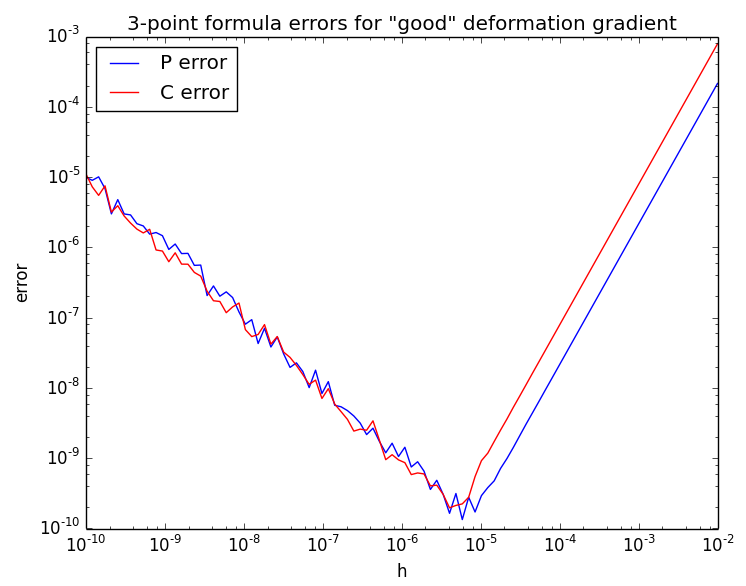
\includegraphics[width=3.25in]{error_good_F.png} \quad
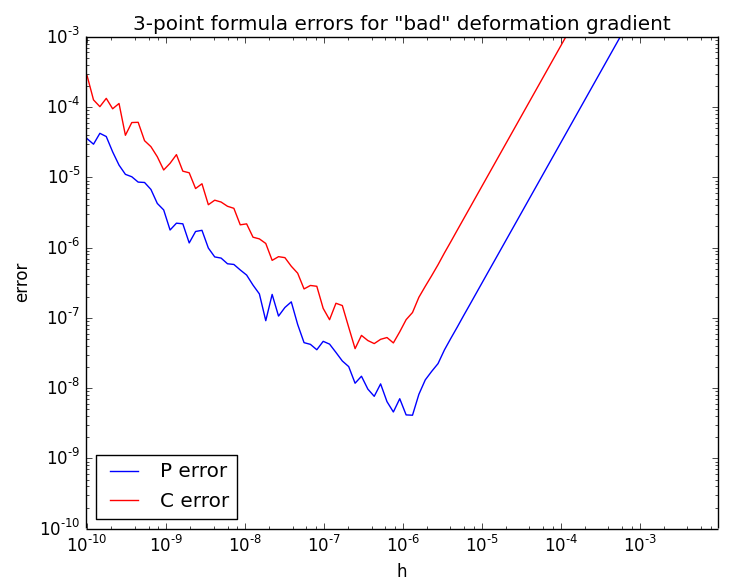
\includegraphics[width=3.25in]{error_bad_F.png} 
\caption{The ``good" deformation gradient yields a smaller error for both the first Piola-Kirchhoff stress and in particular for the tangent moduli. Both plots indicate that the minimum error occurs for a perturbation between $10^{-5}$ and $10^{-6}$.} 
\label{fig: numerical differentiation error}
\end{figure}

In order to find the value of $h$ that gives the minimum errors, I generated 100 random deformation gradients and computed the average error for the stress and for the tangent moduli for several values of $h$ for a custom material with first lam\'e parameter $\lambda = 5$ and shear modulus $\mu = 3$. The results are shown in table \ref{table: h vs. error}.

\begin{table}[h]
	\centering
	\caption{The perturbation $h$ affects the error of the 3-point formula approximation.}
	\begin{tabular}{ | c | c | c | c | c | }
		\hline
		h & Average P Error & Max P Error & Average C Error & Max C Error \Tstrut \\ \hline
		$7.5 \times 10^{-4}$ & $4.4 \times 10^{-6}$  & $1.1 \times 10^{-4}$ & $3.4 \times 10^{-5}$ & $1.2 \times 10^{-3}$ \Tstrut \\
		$1.0 \times 10^{-5}$ & $5.3 \times 10^{-10}$ & $3.7 \times 10^{-9}$ & $2.5 \times 10^{-9}$ & $2.5 \times 10^{-8}$ \\
		$2.5 \times 10^{-5}$ & $5.8 \times 10^{-9}$  & $1.9 \times 10^{-7}$ & $4.9 \times 10^{-8}$ & $2.4 \times 10^{-6}$ \\
		$5.0 \times 10^{-5}$ & $4.9 \times 10^{-8}$  & $3.4 \times 10^{-6}$ & $7.7 \times 10^{-7}$ & $6.7 \times 10^{-5}$ \\
		$7.5 \times 10^{-5}$ & $6.1 \times 10^{-8}$  & $3.0 \times 10^{-6}$ & $6.5 \times 10^{-7}$ & $4.8 \times 10^{-5}$ \\
		$\bm{1.0 \times 10^{-6}}$ & $\bm{1.4 \times 10^{-9}}$  & $\bm{2.9 \times 10^{-9}}$ & $\bm{1.2 \times 10^{-9}}$ & $\bm{4.0 \times 10^{-9}}$ \\
		$2.5 \times 10^{-6}$ & $6.2 \times 10^{-10}$ & $1.5 \times 10^{-9}$ & $9.0 \times 10^{-10}$& $1.8 \times 10^{-8}$ \\
		$5.0 \times 10^{-6}$ & $3.3 \times 10^{-10}$ & $1.7 \times 10^{-9}$ & $8.4 \times 10^{-10}$& $1.6 \times 10^{-8}$ \\
		$7.5 \times 10^{-6}$ & $5.8 \times 10^{-10}$ & $1.5 \times 10^{-8}$ & $3.9 \times 10^{-9}$ & $1.7 \times 10^{-7}$ \\
		\hline
	\end{tabular}
\label{table: h vs. error}
\end{table}

Based on figure \ref{fig: numerical differentiation error} and table \ref{table: h vs. error}, the default value for the perturbation $h$ was selected to be $10^{-6}$ because it seems to provide consistently small average and maximum errors for both the stress and tangent moduli. $h$ is included as an optional parameter in the verification test functions that can be specified if desired. Note that the absolute value of these errors can be affected by the material properties by several orders of magnitude. This will be examined further in the discussion section of the report.

\subsection{Verification Tests}
The material frame indifference and material symmetry tests are performed on random deformation gradients to check for the validity of the constitutive model. Typical results for the quantities defined in section \textit{\nameref{sec: verification tests}} are shown in tables \ref{table: material frame indifference} and \ref{table: material symmetry}.

% TODO gaussian quadrature vs. exact integration. Make table for order and element type, error. 

% TODO rank tests for stiffness matrix, meaning and expected values. 

% TODO comment on results for each of the above

\begin{table}[h]
	\centering
	\caption{Typical results of material frame indifference tests.}
	\begin{tabular}{ | c | c | }
		\hline
		Quantity & Max Error \Tstrut \\ \hline
		$w$ 		& $1.4 \times 10^{-14}$ \Tstrut \\
		$\bm{P}$ 	& $3.6 \times 10^{-15}$ \\
		$\bm{C}$ 	& $4.3 \times 10^{-14}$ \\
		\hline
	\end{tabular}
	\label{table: material frame indifference}
\end{table}

\begin{table}[h]
	\centering
	\caption{Typical results of material symmetry tests.}
	\begin{tabular}{ | c | c | }
		\hline
		Quantity & Max Error \Tstrut \\ \hline
		$w$ 		& $2.8 \times 10^{-14}$ \Tstrut \\
		$\bm{P}$ 	& $1.4 \times 10^{-14}$ \\
		$\bm{C}$ 	& $2.1 \times 10^{-14}$ \\
		\hline
	\end{tabular}
	\label{table: material symmetry}
\end{table}

These quantities should be exact matches, so the only error here is due to loss of precision from floating point operations. These operations give 16 digits of accuracy, which is why we see errors only in the last few digits on the order of $10^{-13}$ to $10^{-15}$ depending on the order of magnitude of the quantity itself.  

\subsection{Tolerance}
We want to determine the smallest possible tolerance value for which all of our tests will pass. The numerical differentiation test is really the limiting factor here, and as these errors are determined by the quality of the approximation formula, unlike the material tests which provide nearly exact answers only limited by 16-digit precision. The numerical differentiation tests involve expressions that contain material properties $\lambda$ and $\mu$, and therefore the error will actually vary as a function of these parameters as well. The code will raise an exception in the case were the error of the numerical approximation exceeds the tolerance. In order to determine a tolerance value that will work for all materials, 100 tests were run using random deformation gradients for 3 materials, and the exceptions were counted for a given tolerance. One of the materials is a custom material, with $\lambda = 6$ and $\mu = 3$, and the other two are aluminum alloy and glass. The results are shown in table \ref{table: tolerance}. 

\begin{table}[h]
	\centering
	\caption{Number of exceptions for 3 materials at various tolerance values out of 100 runs.}
	\begin{tabular}{ | c | c | c | c | c |}
		\hline
		Tolerance  & \# of Exceptions (Custom) & \# of Exceptions (Al) & \# of Exceptions (Glass) & \# of Runs \Tstrut \\ \hline
		$10^{-6}$  & 0   & 0   & 0   & \ 100 \Tstrut \\
		$10^{-7}$  & 0   & 2   & 1   & 100 \\
		$10^{-8}$  & 0   & 64  & 25  & 100 \\
		$10^{-9}$  & 81  & 100 & 100 & 100 \\
		$10^{-10}$ & 100 & 100 & 100 & 100 \\
		\hline
	\end{tabular}
	\label{table: tolerance}
\end{table}

%%%%%%%%%%%%%%%%%%%%%%%%%%%%%%%%%%%%%%%%%%%%%%%%%%%%
\section{DISCUSSION AND CONCLUSIONS}
\label{sec: discussion}

The code has been thoroughly tested for over 10,000 random deformation gradients (all of which were checked to be physical) using several different materials such as aluminum alloy, lead, and glass, as well as custom materials. All verification tests pass as well as the numerical differentiation checks. The passing of material frame indifference and material symmetry implies that the constitutive law is implemented correctly, as the quantities behave appropriately under random rotations. These tests yield exact results limited only by the 16-digit precision of floating point operations. 

The passing of the numerical differentiation tests, using the 3-point formula, implies that the computed quantities that come from derivatives of the deformation gradient, namely the first Piola-Kirchhoff stress and the tangent moduli, are within tolerance of the values that result from Taylor Expansion. Whether these checks pass is largely determined by the tolerance value chosen. As discussed previously, the perturbation value $h$ used in the 3-point formula has been selected such that the error is consistently minimized (see \ref{table: h vs. error}). However, the absolutely value of this error is affected by the material selected, because the material properties are used in the expression for the stress and tangent moduli. Based on the results in table \ref{table: tolerance}, as well as some additional testing, I have chose a tolerance of $10^{-6}$, because this value consistently results in 0 exceptions for every material tested, while $10^{-7}$ will occasionally result in an error or two. I could perform further testing at finer intervals than factors of 10, but this will provide an adequate starting point. It should be noted that while the derivation of the 3-point formula implies that errors should scale with $h^2$, which is indicated by the slope of 2 on the log-log plots shown in figure \ref{fig: numerical differentiation error}. 


%%%%%%%%%%%%%%%%%%%%%%%%%%%%%%%%%%%%%%%%%%%%%%%%%%%%
\section{SOURCE CODE LISTING}

\begin{tabular}{ r l }
\textit{New and updated files:} & body.py, constants.py, constitutive\_models.py, exceptions.py, frames.py, \\
					  & kinematics.py, materials.py, model.py, model\_io.py, operations.py, tests.py 
\end{tabular}

\end{document} 
